\newpage 
\setcounter{page}{1}

\chapter{序論}

\section{研究背景}
近年ハードやソフトの技術進歩により, 3 Dimensional Computer Graphics(3DCG)の表現力が向上している.特にゲームやメタバースなどの開発においては詳細な表現から広大なマップまで,高いクオリティが求められることも多くなっている.そのため大規模な開発では数年かかることも多くなっている.そこで, 3DCG 開発においてプロシージャルモデリングという手法がよく利用されている.プロシージャルモデリングとは,数式などの処理を組み合わせてモデリングを行う手法であり,計算処理を設計後は,あらかじめ設定された複数の説明変数のパラメータを変更するだけで様々なモデルを生成する事が出来る手法である.開発者以外がプロシージャルモデリングに触れる機会として,ゲームのキャラクタークリエイトが挙げられる.身長や体格,顔の位置といった様々な値を変更することでプレイヤーの好きなキャラクターを作成する事が出来る.図\ref{fig:metahuman_cc1}に MetaHuman\footnote{\url{https://www.unrealengine.com/en-US/metahuman}}によるキャラクタークリエイトを示す.一方で前述の通り表現力の向上から,操作するパラメータの個数が増えてきていることはキャラクタークリエイトにおける調整を行う事が出来るパラメータ数の向上具合から見ても明らかである.図\ref{fig:blenderSFT}に Blender\footnote{\url{https://www.blender.org/}} によるプロシージャルモデリングの様子を示す.画像右側に並んでいるのが操作する事が出来るパラメータであり,このモデルではおよそ30個存在するため,画面上に収まっていない.パラメータの個数が増えることはその分一つのオブジェクトにかける開発時間の増加を伴う.加えて,コンテンツ自体の内容量が増加しているためモデリングを行うオブジェクトの数も増加傾向にあるので,開発時間の増大が著しい.そこで本研究では,モデリング時間の短縮のために操作するパラメータ数の多さに着目し,パラメータ数の削減によってモデリング時間短縮を試みる. 


複数のパラメータを操作し適したモデリングを行うというのは,開発者の考える最適なパラメータを設定するという点で組み合わせ最適化問題として捉える事が出来る.そこでメタヒューリスティクスで組み合わせ最適化問題に有効な手法としてユーザとの対話が可能なインタラクティブ遺伝的アルゴリズムを用いてモデル提案を行うことで効率的な探索を行えることを期待する.


\begin{figure}[h]
	\begin{center}
		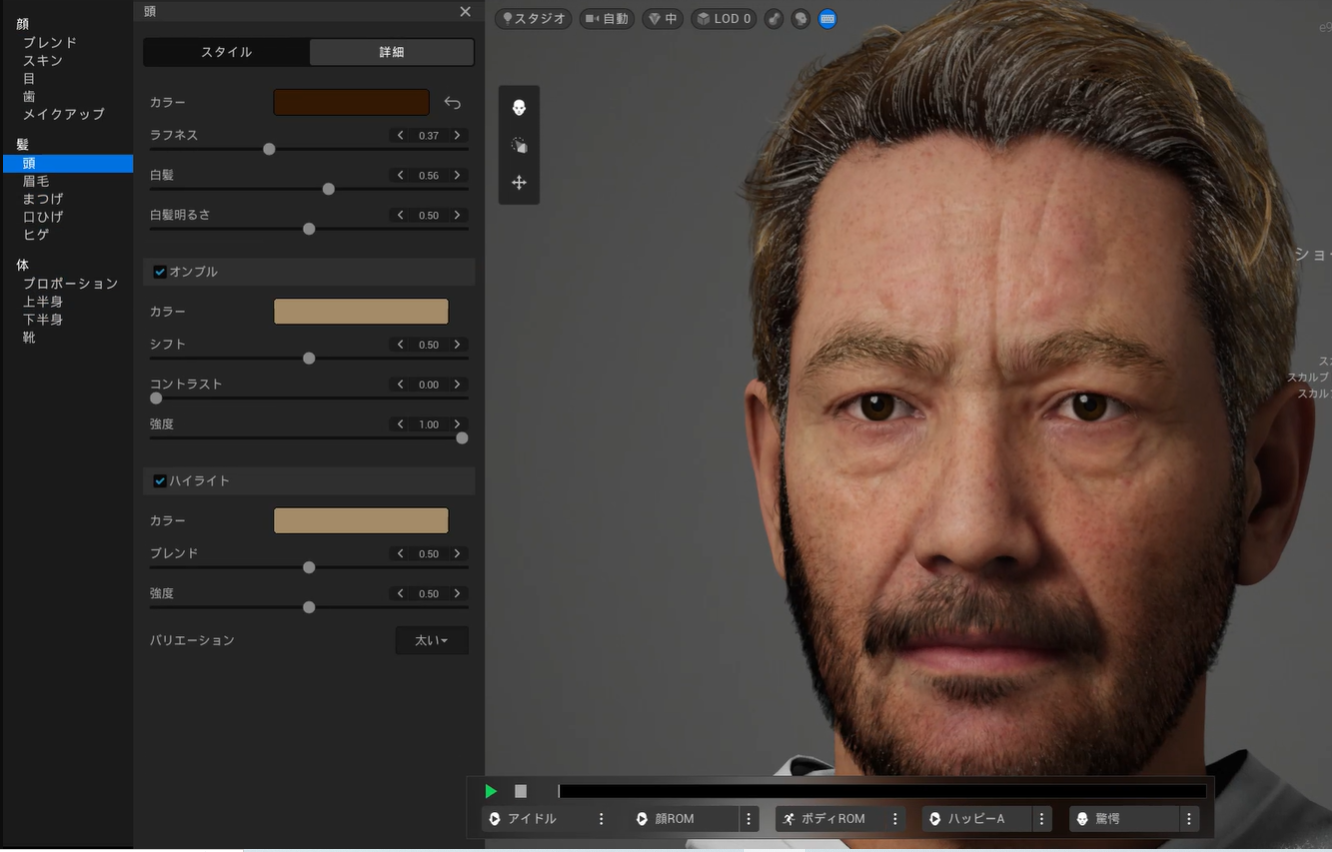
\includegraphics[scale=0.4]{./imgs/metahuman1.PNG}
		\caption[MetaHuman におけるキャラクター作成]{MetaHuman \hyperref[fn:3]{\footnotemark[3]}におけるキャラクター作成\label{fig:metahuman_cc1}}
	\end{center}
\end{figure}

\footnotetext[3\label{fn:3}]{\url{https://metahuman.unrealengine.com/}}

\begin{figure}
	\begin{center}
		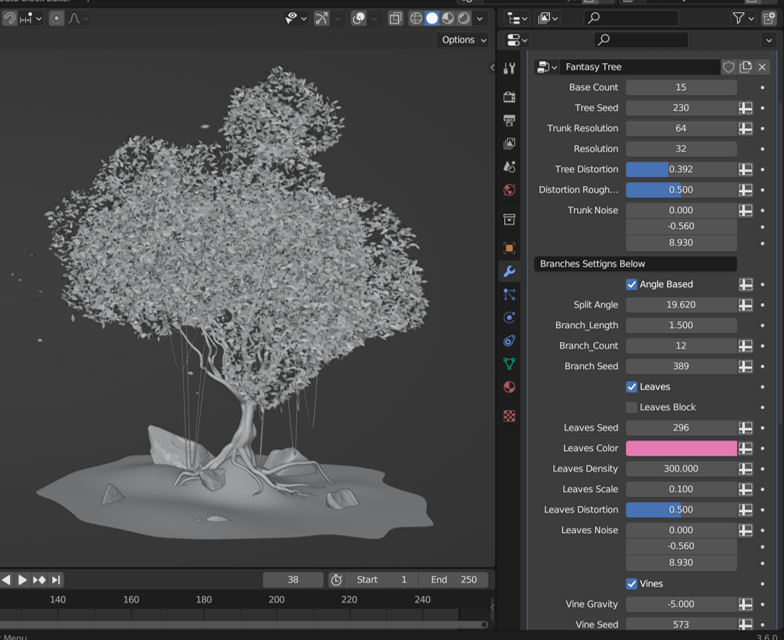
\includegraphics[scale=0.5]{./imgs/blenderSFT.PNG}
		\caption{Blender におけるプロシージャルモデリング\label{fig:blenderSFT}}
	\end{center}
\end{figure}

\newpage
\section{研究目的}
    本研究では,プロシージャルモデリングにおいて制作時間短縮を目的とし,インタラクティブ遺伝的アルゴリズムを利用した操作パラメータ数を削減したシステムを提案し,ユーザ実験を通して検証を行う.操作パラメータ削減によって制作時間短縮だけでなくユーザビリティの向上に繋げることも目的とする.



\section{論文構成}
    本論文は5章で構成する.まず,2章では要素技術および関連研究について紹介する.続いて3章で実験手法の提案をし,4章において実験結果と考察を示す.5章で本研究の成果をまとめた上で,今後の課題について述べる.
